\documentclass[../../main]{subfiles}
\begin{document}

\subsection{Application architecture}
\label{ss:application-architecture}

Our application is designed to have many modules, each of them with its own duty, to enable users of \textbf{SocialPlaces} to perform all the possible things they can do with the system.\\
An overview of the application can be seen in the following diagram:
\begin{figure}[h]
    \centering
    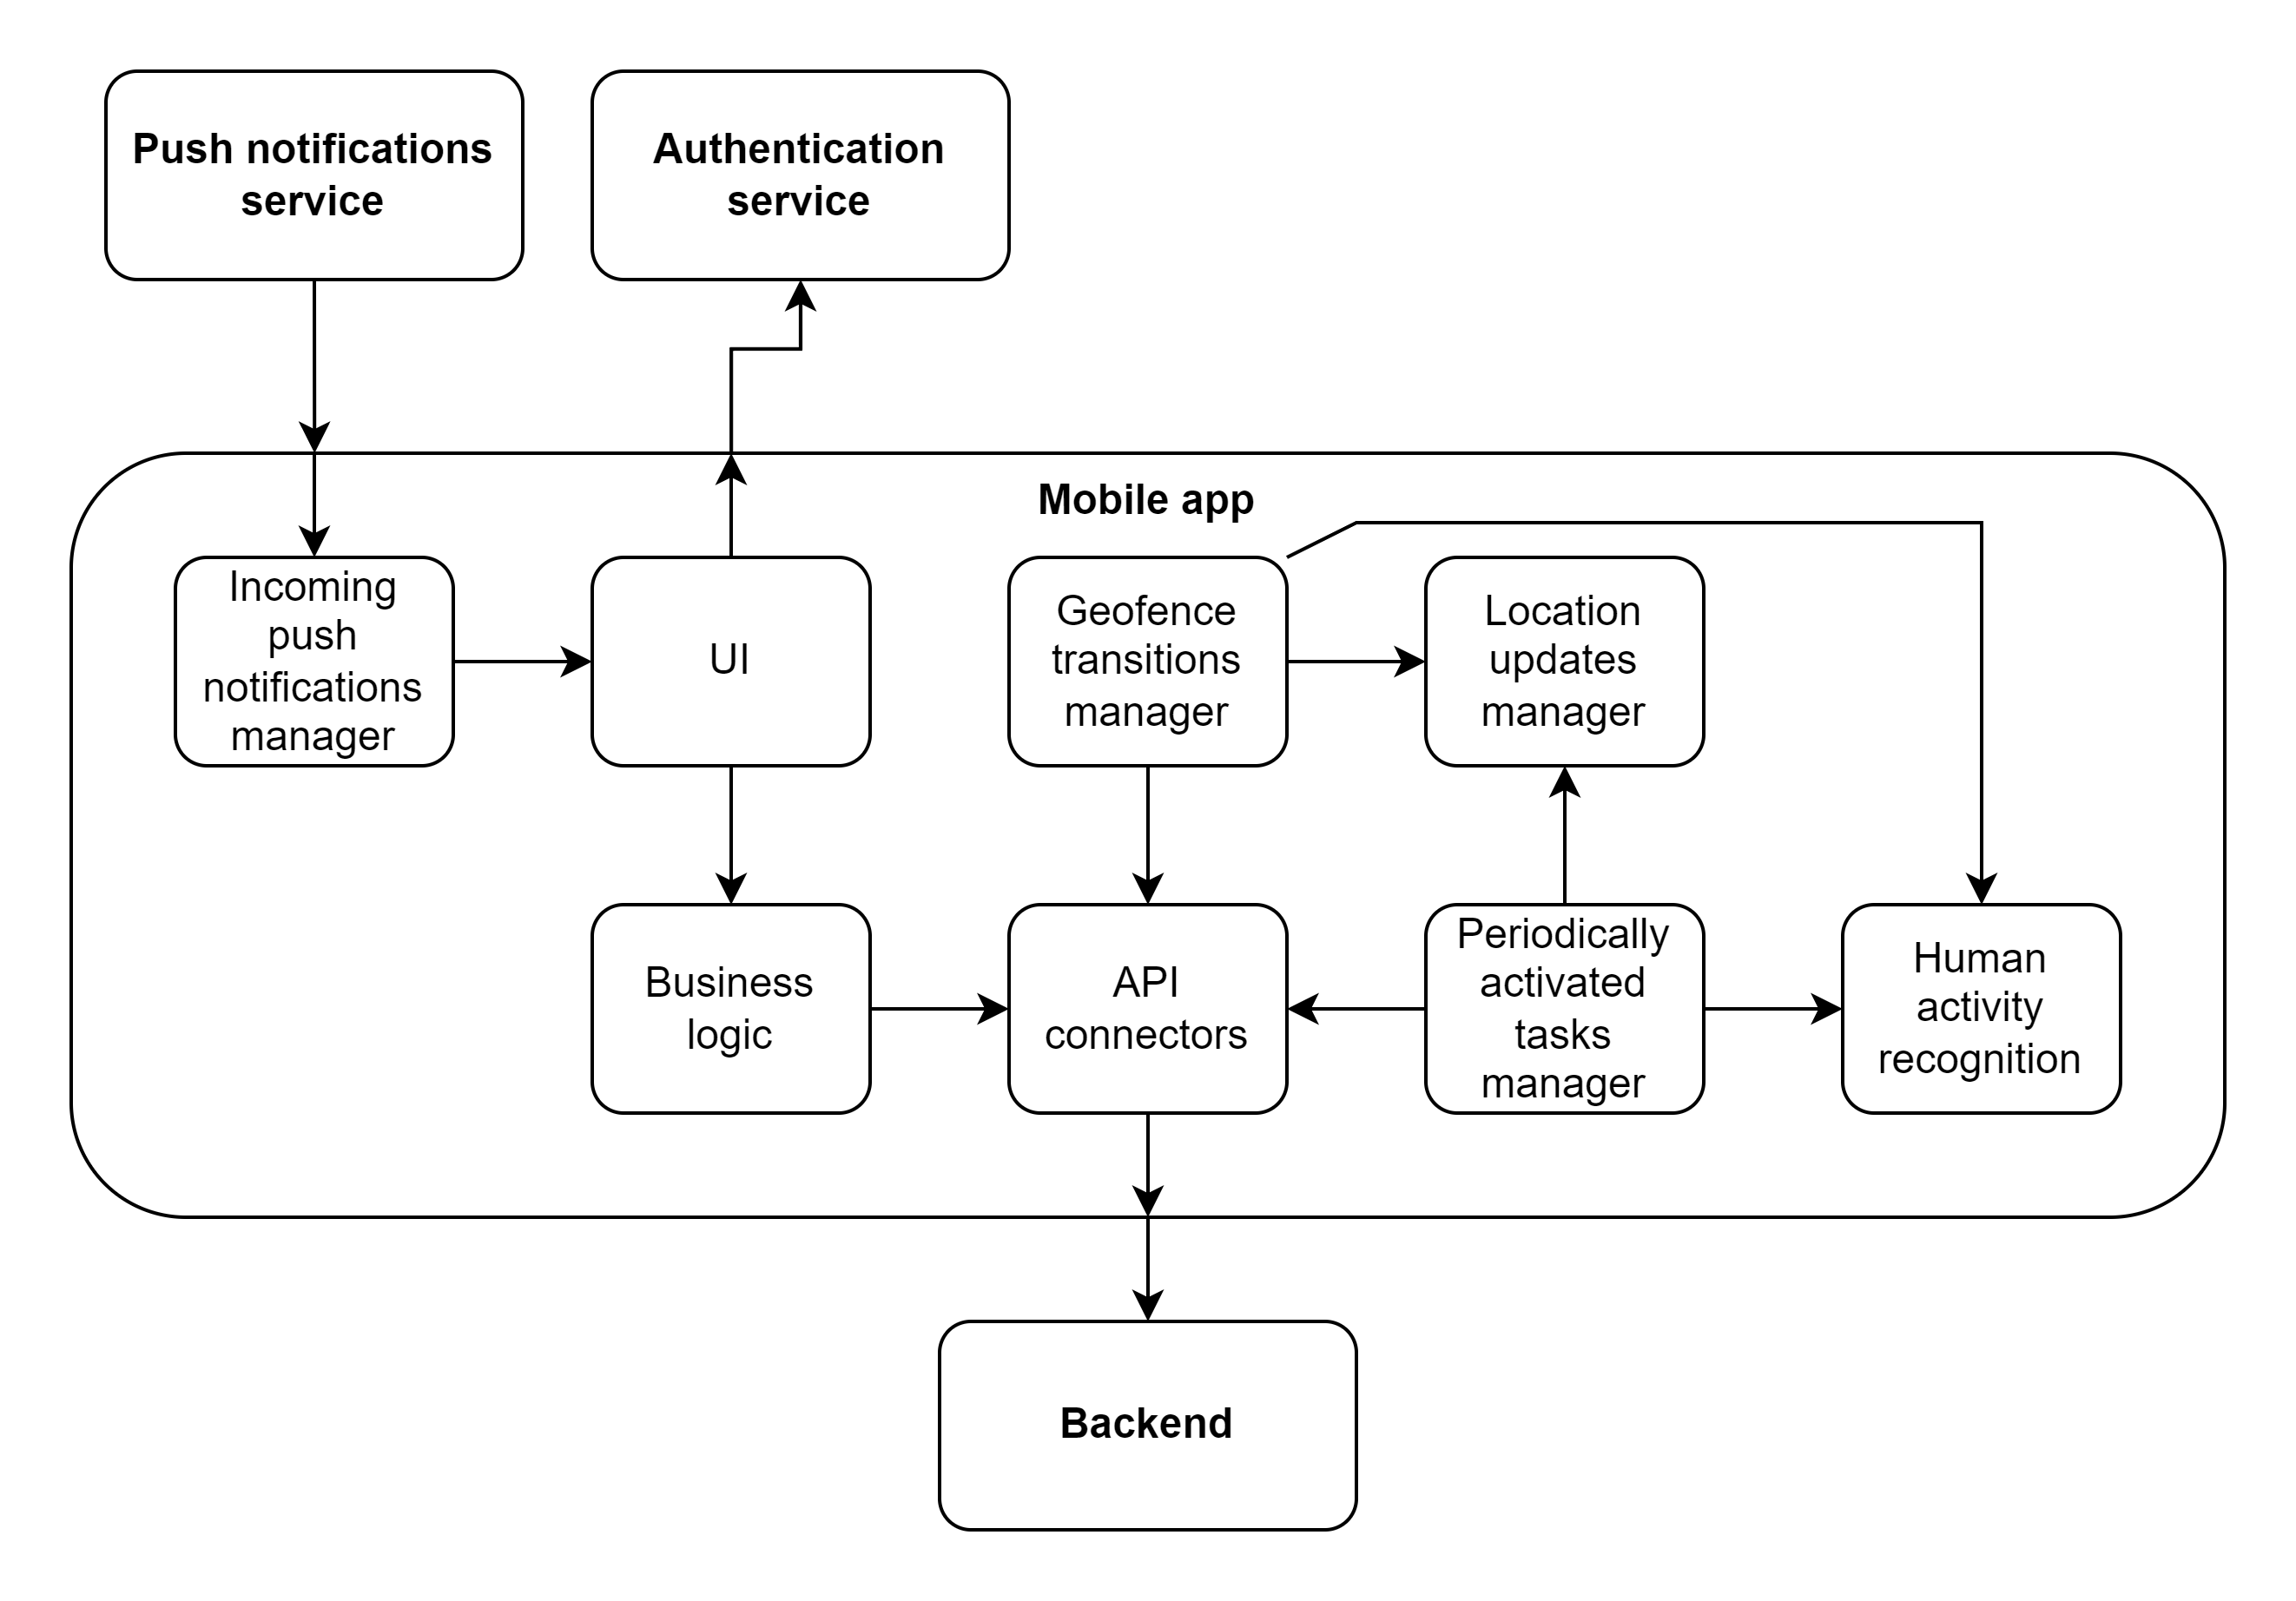
\includegraphics[width=0.65\textwidth]{images/application_architecture}
    \caption{Application architecture}\label{img:application_architecture}
\end{figure}\\
\noindent
Let's now focus more in detail to what purpose each of the parts in the diagram (and hence, in the application) has:
\begin{itemize}
    \item \textbf{UI}, the user interface handles all the interactions coming from the user and communicates results and errors accordingly;
    \item \textbf{Business logic}, the business logic or \textit{domain} aims at being an interface between the high-level requests coming from the UI module and those that have to be forwarded to the backend of the system via its APIs;
    \item \textbf{API connectors}, it works as a bridge between the requests coming from the different modules of the application and the APIs exposed by the backend;
    \item \textbf{Geofence transitions manager}, allows the application to be notified by the operating system when the device finds itself inside a \textit{geofence} of a \textit{poi} owned by the user;
    \item \textbf{Location updates manager}, allows the application to be notified by the operating system when the device's GPS sends a location update, i.e. when a new pair \textit{(latitude, longitude)} is available (crucial for all the types of recommendations directed to the user);
    \item \textbf{Periodically activated tasks manager}, allows the execution of certain tasks after a certain amount of time, previously set, has passed. It is used for periodic recommendations;
    \item \textbf{Human activity recognition}, allows to get the current human activity of a user, requesting it to the device's sensors enabled for this purpose;
    \item \textbf{Incoming push notifications manager}, allows to receive notification by the \textbf{Push notification service} and handles them accordingly.
\end{itemize}
As we mentioned in the previous section, these modules are developed by us, and we decided to make use of external services for authentication and notification purposes.\\
The \textbf{Authentication service} is called during the application start-up in order to receive rights to send requests to the backend of the system through its APIs.
The \textbf{Push notifications service} notifies the module of the application that handles push notifications, sending all the data to fulfil what the application needs to do.

\end{document}